\documentclass[11pt]{article}
\usepackage{graphicx}
\usepackage{float}

\title{Laborator 1 - SO}
\author{Rus Lucian-Florin}
\date{March 19, 2026}

\begin{document}

\maketitle


\newpage
\section*{Comenzi laborator}

\begin{figure}[H]
    \centering
    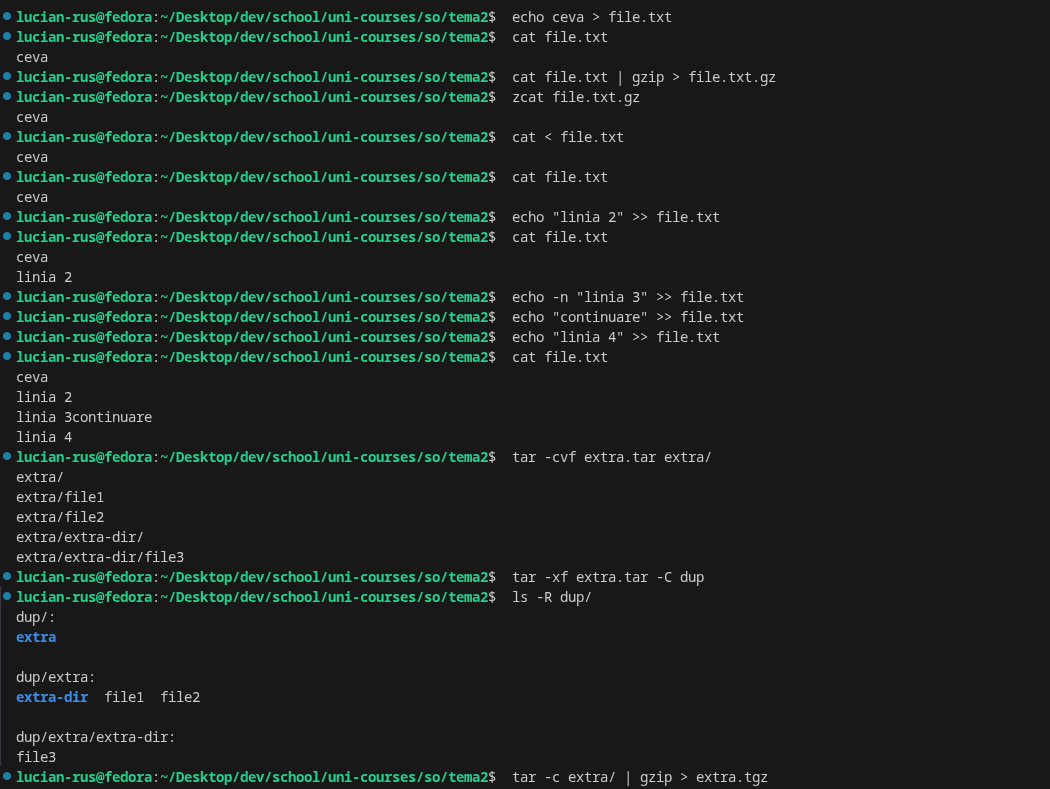
\includegraphics[width=0.8\textwidth]{1.png}
\end{figure}

\begin{figure}[H]
    \centering
    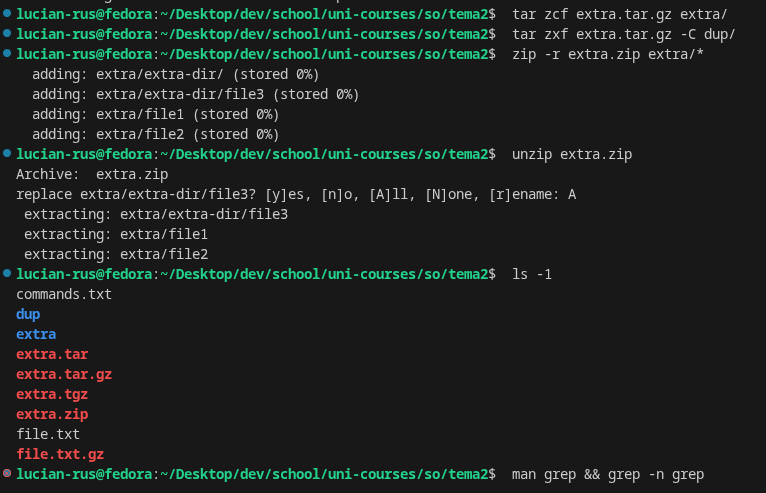
\includegraphics[width=0.8\textwidth]{2.png}
\end{figure}

\begin{figure}[H]
    \centering
    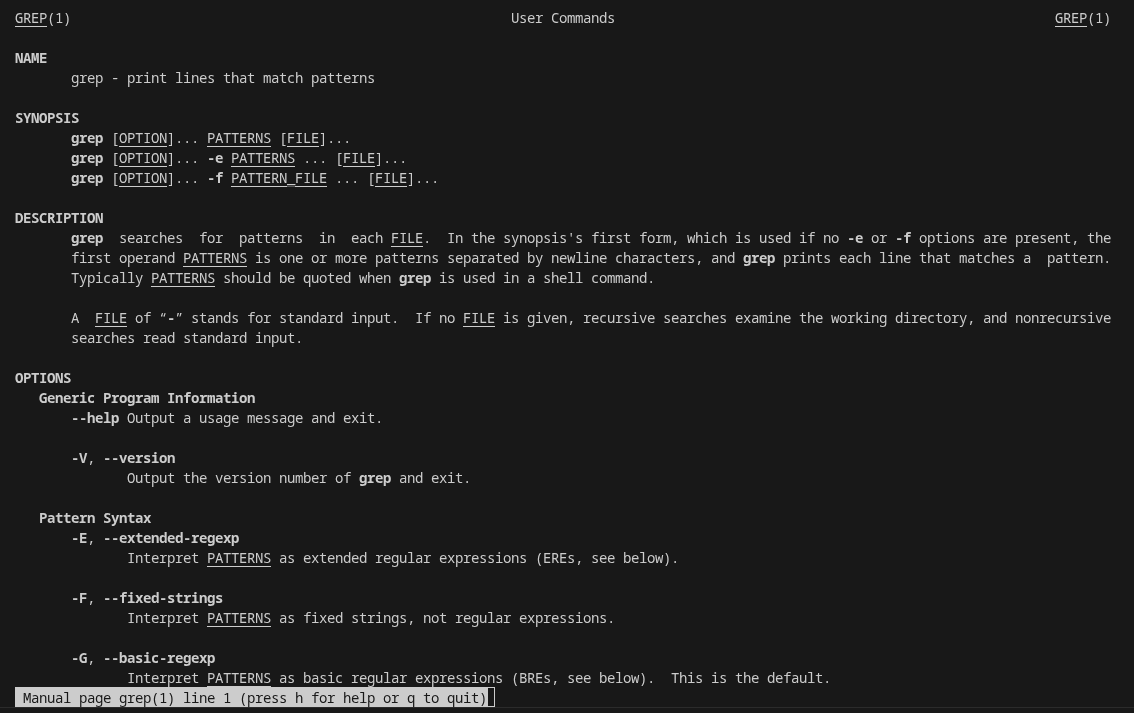
\includegraphics[width=0.8\textwidth]{3.png}
\end{figure}

\begin{figure}[H]
    \centering
    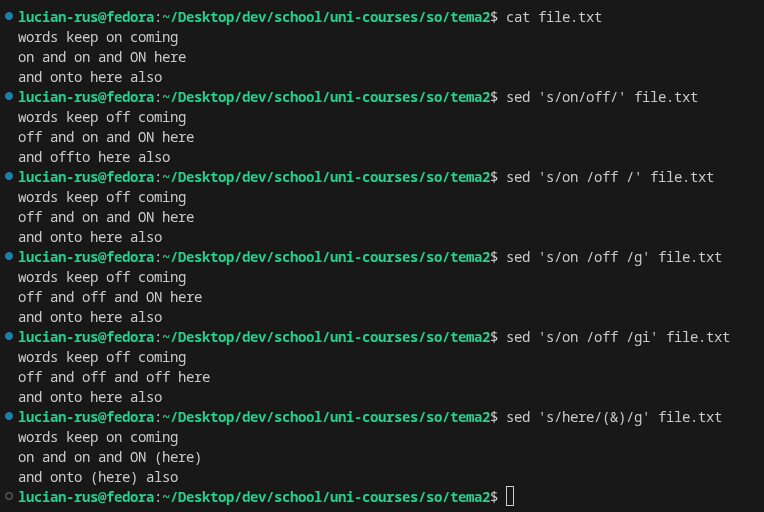
\includegraphics[width=0.8\textwidth]{4.png}
\end{figure}

\newpage
\begin{figure}[H]
    \centering
    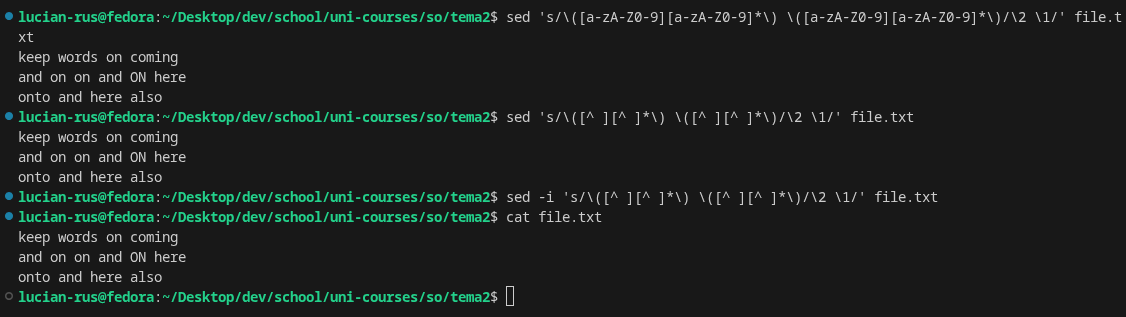
\includegraphics[width=0.8\textwidth]{5.png}
\end{figure}

\begin{figure}[H]
    \centering
    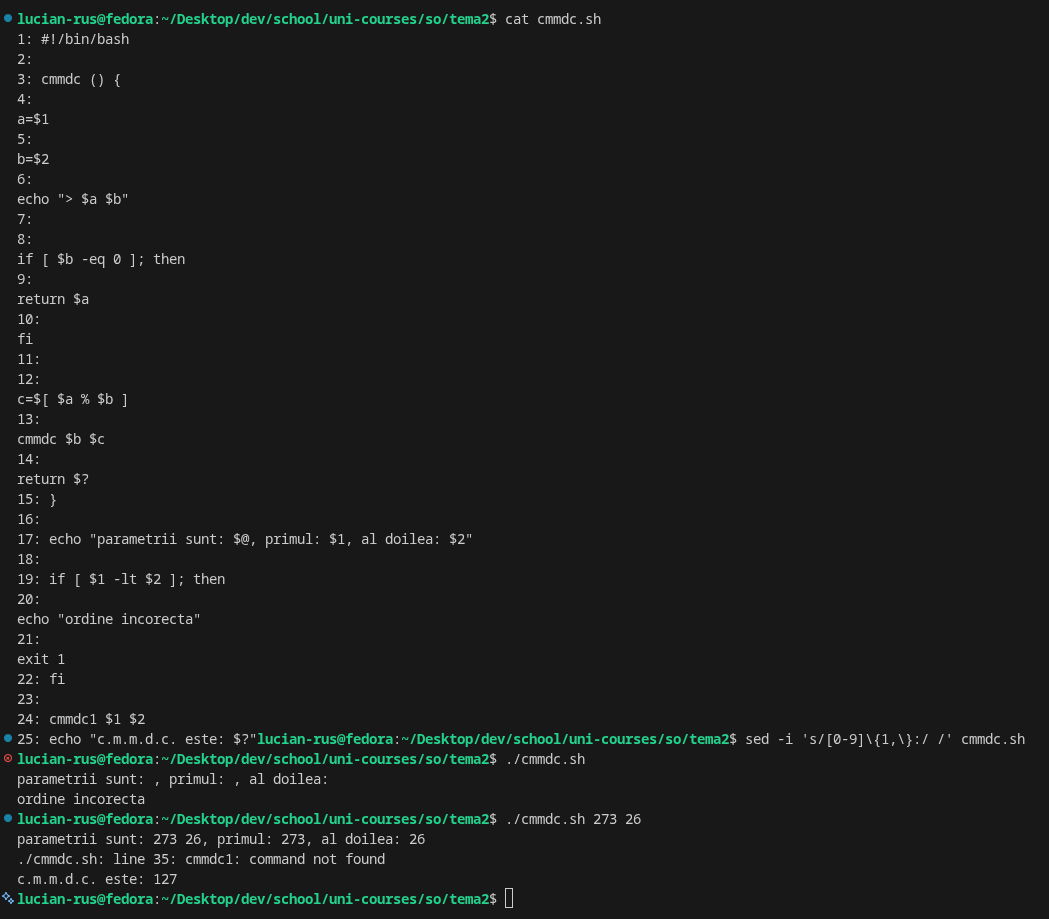
\includegraphics[width=0.8\textwidth]{6.png}
\end{figure}

\section*{Teme}

\begin{figure}[H]
    \centering
    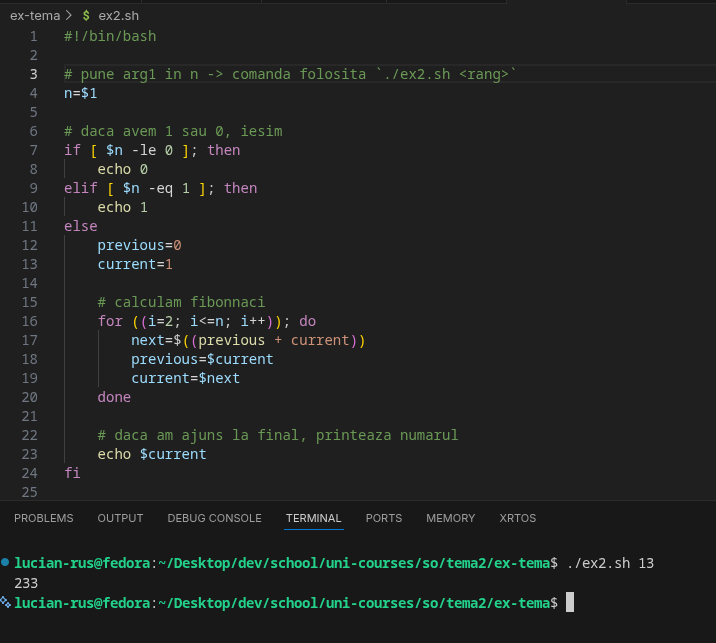
\includegraphics[width=0.8\textwidth]{7.png}
    \caption{Exercitiul 2}
\end{figure}

Determinarea termenului Fibonnaci de rang n. Operatii efectuate:
\begin{itemize}
  \item daca n = 0, printam numarul
  \item daca n = 1, printam numarul
  \item calculam termenul Fibonnaci prin utilizarea unui \textbf{for} loop 
\end{itemize}

\begin{figure}[H]
    \centering
    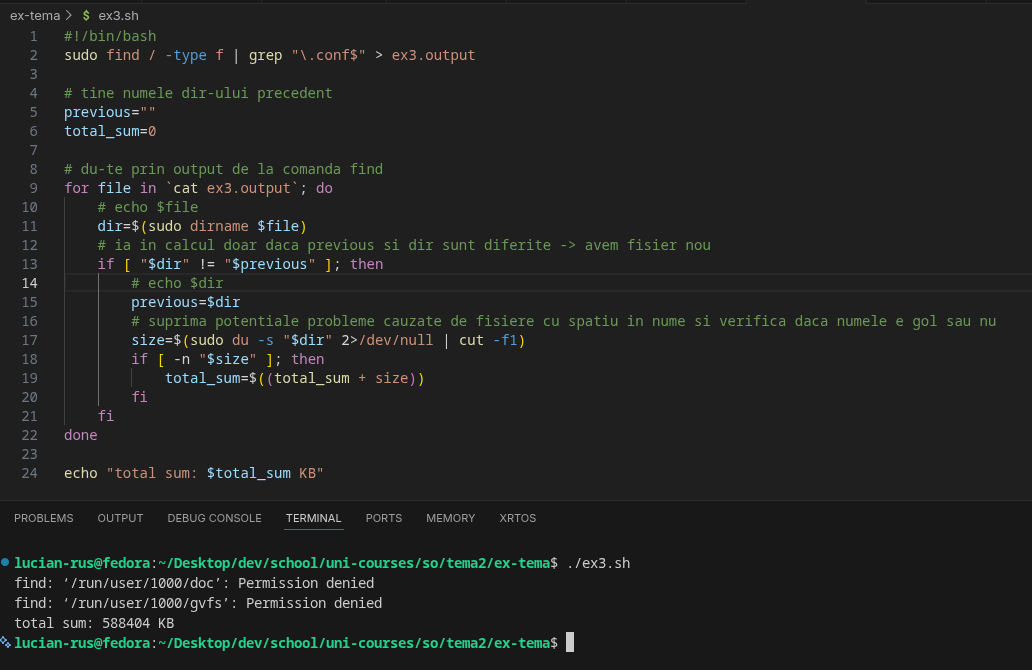
\includegraphics[width=0.8\textwidth]{8.png}
    \caption{Exercitiul 3}
\end{figure}

Determinarea sumei dimensiunilor tuturor directoarelor care contin fisiere de configuratii (fisiere terminate in \textbf{.config}). Operatii efectuate:
\begin{itemize}
  \item listam toate fisierele care se termina in \textbf{.conf} folosind \textbf{find} si \textbf{grep} si salvam continutul intr-un fisier
  \item iteram prin continutul fisierului rezultat si extragem directorul in care se afla fisierele utilizand comanda \textbf{dirname}
  \item verificam daca directorul curent e diferit de cel precedent; acest lucru ne ajuta sa evitam fisierele duplicat
  \item daca fisierul nu e duplicat, determinam dimensiunea lui folosind comanda \textbf{du}; aditional, facem o verificare pentru preventia erorilor generate de directoarele cu spatii in nume
  \item cumulam dimensiunea in variabila \textbf{total\_sum} si o afisam la final
\end{itemize}

\newpage
\begin{figure}[H]
    \centering
    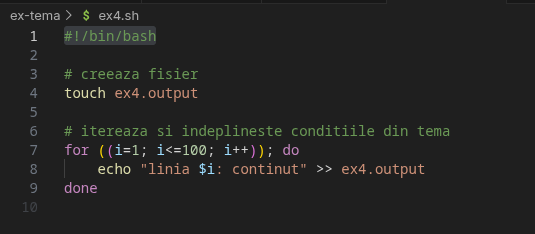
\includegraphics[width=0.8\textwidth]{9.png}
    \caption{Exercitiul 4}
\end{figure}

\begin{figure}[H]
    \centering
    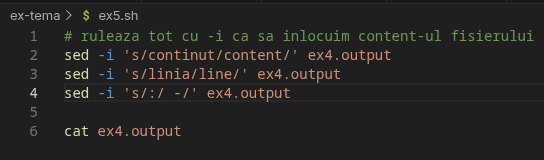
\includegraphics[width=0.8\textwidth]{10.png}
    \caption{Exercitiul 5}
\end{figure}

Generarea unui fisier si alterarea continutului sau. Operatii facute:
\begin{itemize}
  \item cream un fisier gol folosind comanda \textbf{touch}
  \item cream continutul cerut de exercitiu cu ajutorul unui loop \textbf{for}; fiecare linie contine indexul la care se afla; numerotarea incepe de la 1
  \item inlocuim continutul in interiorul fisierului utilizand comanda \textbf{sed} si flag-ul \textbf{-i}
  \item listam continutul fisierului folosind \textbf{cat}
\end{itemize}

Explicatia acopera atat exercitiul 4 cat si exercitiul 5.

\end{document}
